\subsection{Hardware Design}
The design of the hardware was developed in such a way that it allowed for continuous azimuth rotation, independent elevation control, and constant RSSI sampling during motorization. Attention was paid to creating a mechanically rigid, electronically isolated, and modular system for power delivery, signal processing, and actuation.

\subsubsection{Mechanical Configuration and Structural Design}

The physical layout of the hardware is arranged into three distinct layers forming a vertical stack: the Power Deck, Logic Deck, and rotating Top Floor.

\textbf{Stationary Foundation (Power Deck \& Logic Deck):} The stationary base is composed of two layers: the Power Deck, where the power source resides in the form of a 3S Li-Ion battery pack. The Power Deck uses a dovetail rail system for easy access to the batteries. Power is delivered via a BMS and is made available through an XT60 female connector. This is followed by the Logic Deck, which includes the azimuth actuator, a NEMA 17 bipolar stepper motor.

\begin{figure}[H]
    \vspace{1em} 
    \centering
    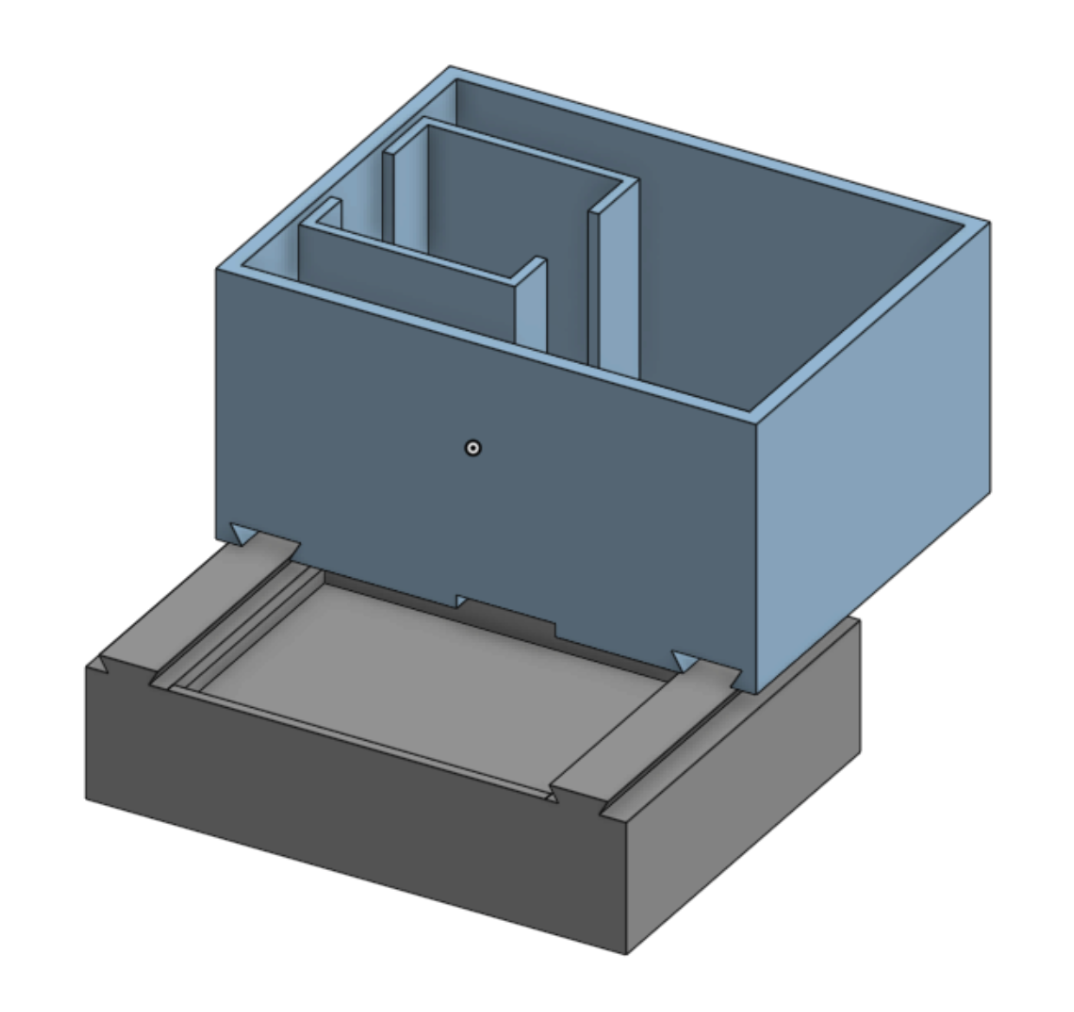
\includegraphics[width=0.6\textwidth]{images/case_design.png}
    \caption{3D Design of the Hardware Enclosure}
    \label{fig:case_design}
\end{figure}

\textbf{Turret Rotation:} The upper rotating section serves as the mounting base for the
controller board (ESP32-S3), tilt actuator (MG90S servo), and antenna components.
The rotational movement of the turret is achieved through the use of a NEMA 17 stepper motor
installed in the static base section, whereas the servo attached to the turret offers the local tilting mechanism for the antenna. In order to solve any potential mechanical problems, a coupling was used to connect the motor shaft to the PCB, resulting in a level surface for the rotor electronics.

\subsubsection{Electromechanical Interface}
To enable continuous 360-degree rotation without cable entanglement, a custom PCB-based slip ring was fabricated. 
This interface manages the transmission of power and logic signals across the rotating boundary.
A PCB-based slip ring was selected over commercial capsule slip rings to reduce
cost, allow custom signal routing, and enable tight integration with the system
mechanical envelope. The design also permits easy modification of ring width and
spacing to improve contact reliability during iterative prototyping.

\textbf{Stator (Bottom Layer):} The stator is made up of a copper-cladded board with four concentric rings that are conductive. The rings represent the necessary channels for data transfer, which include the power source (5V), ground, and digital control signals for the driver of the azimuth motor (STEP and DIR).

\begin{figure}[H]
    \vspace{1.5em} 
    \centering
    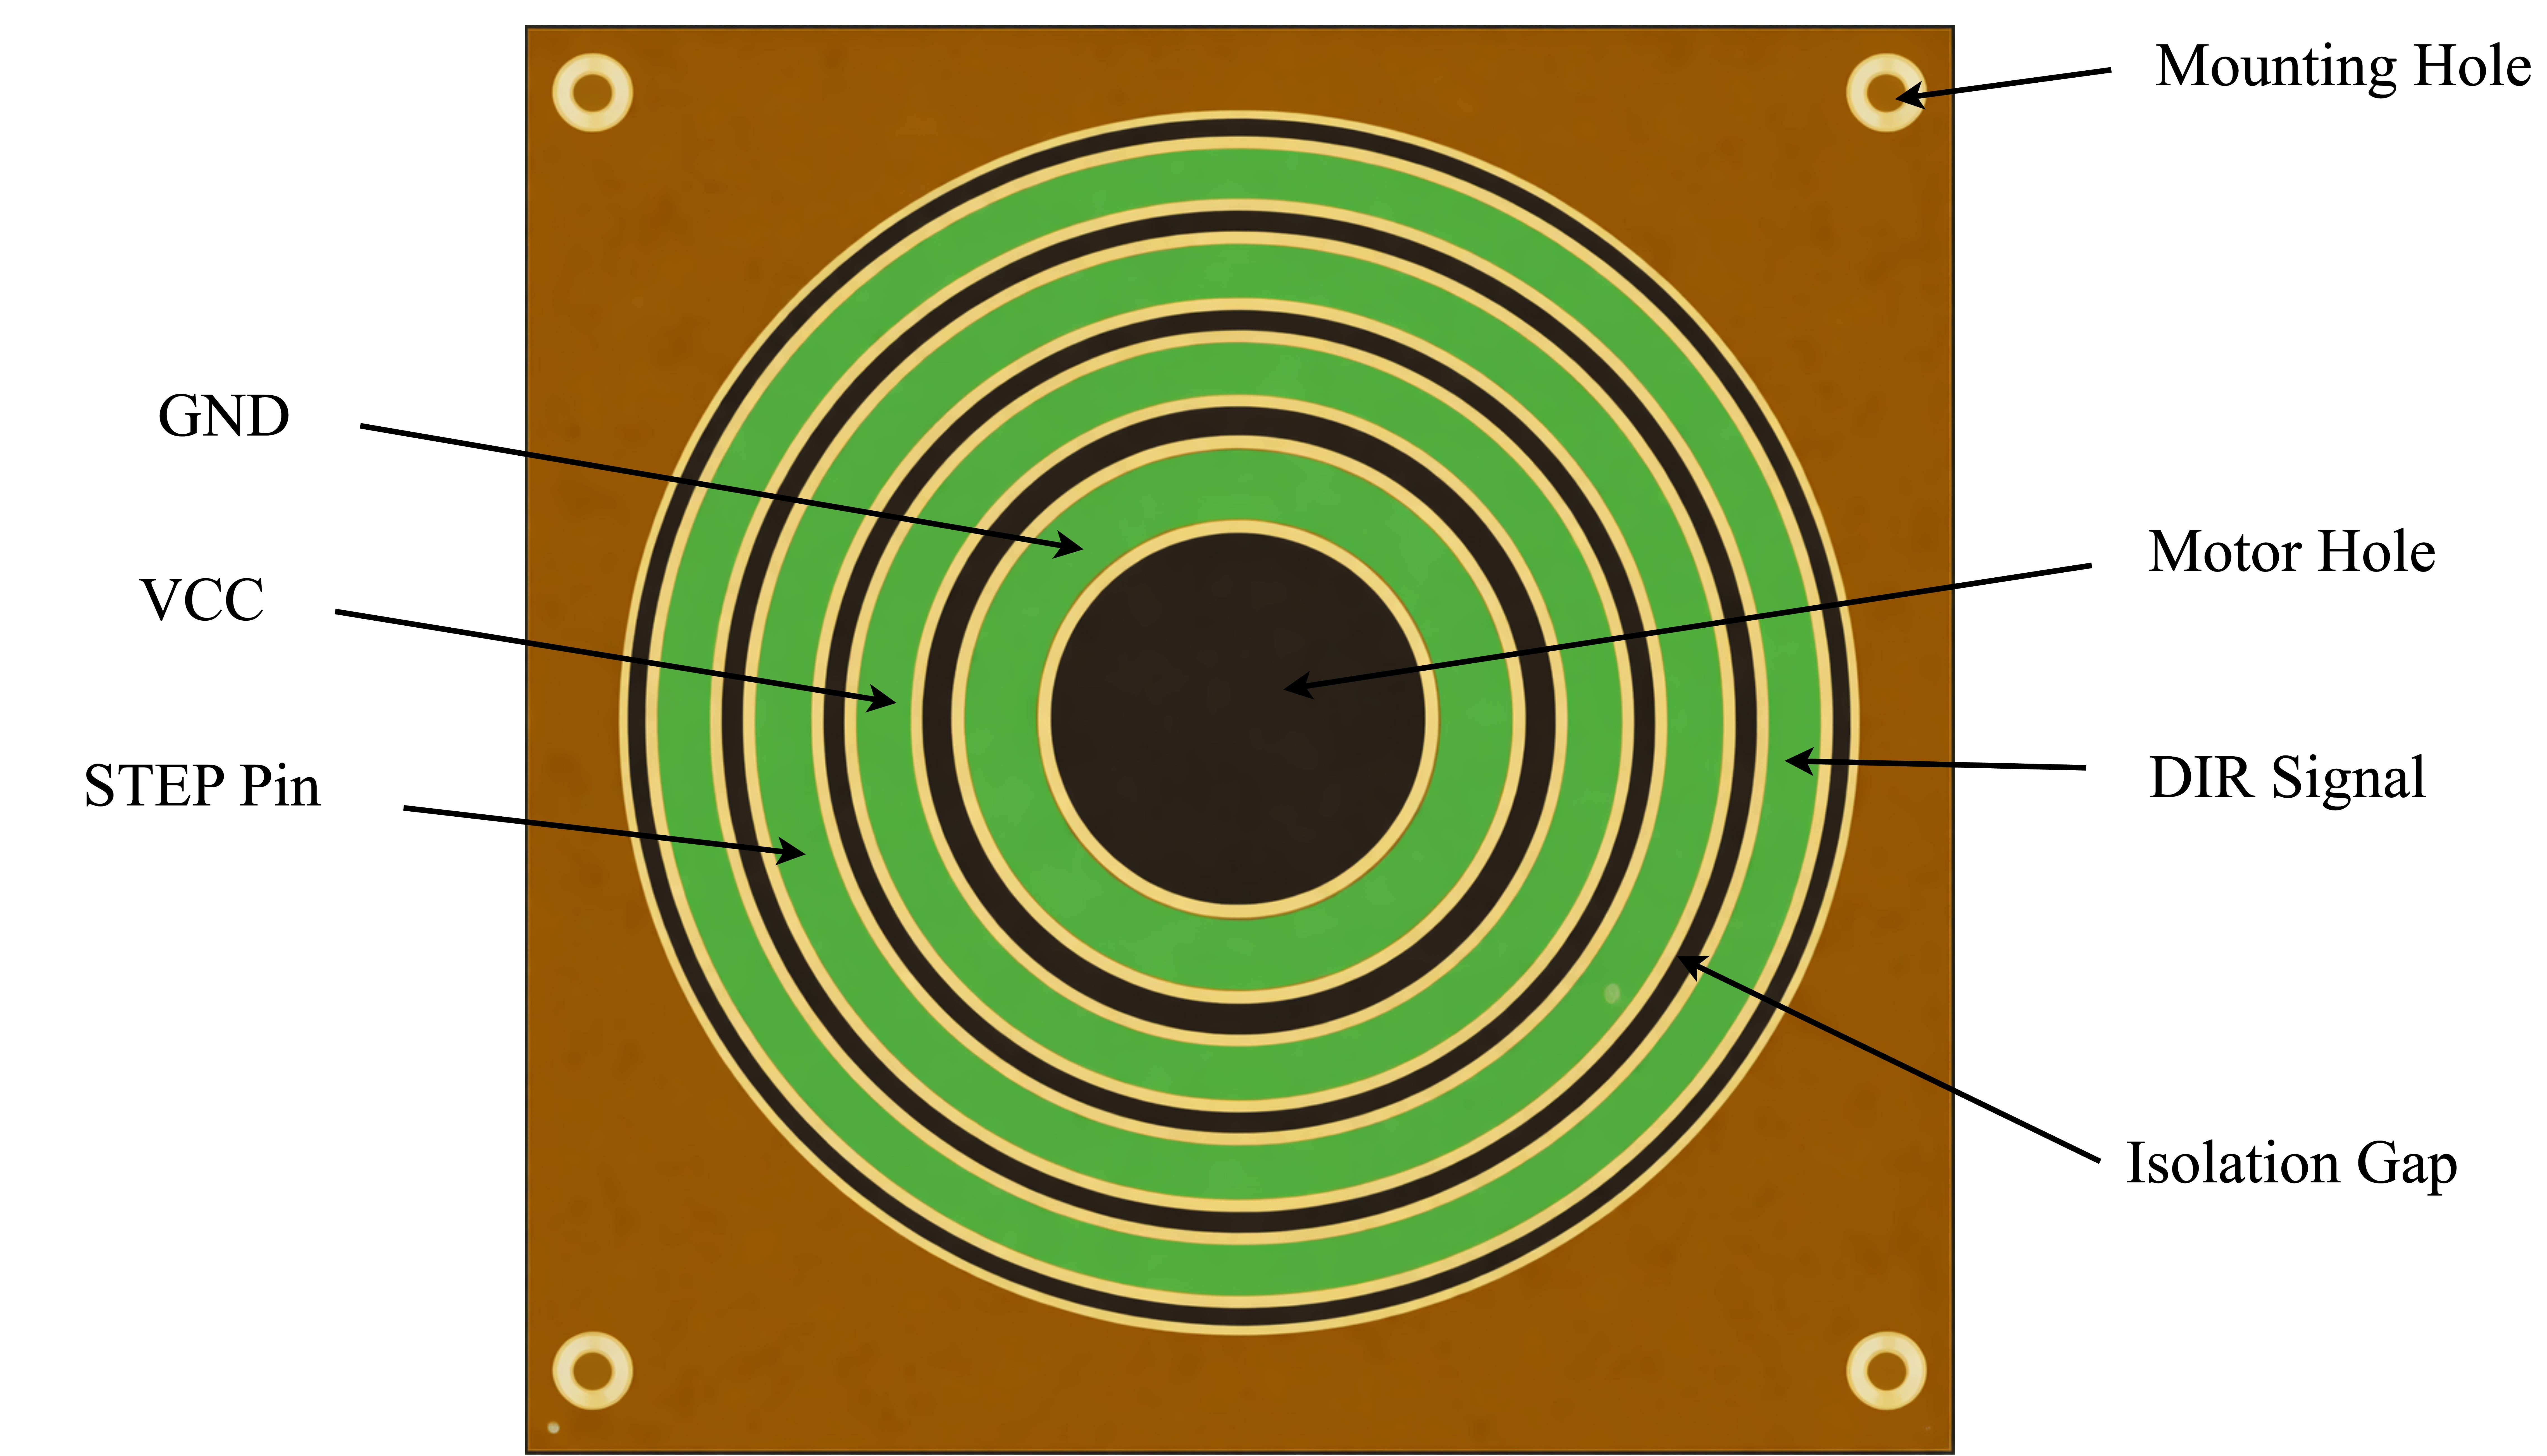
\includegraphics[width=1\textwidth]{images/copper_plate.jpg}
    \vspace{0.15cm}
    \caption{Design of Concentric Copper Plate}
    \label{fig:elect_inteface}
\end{figure}

\textbf{Rotor (Top Layer):} The rotation mechanism involves the use of spring-loaded pogo pins in order to provide continuous electrical connection in case one pin disconnects because of mechanical movement.

\subsubsection{Control Electronics and Circuitry}

The system uses a 3S Li-Ion battery pack supplying a nominal 12V power rail. A 12V rail is used to power the stepper motor directly using the A4988 driver module mounted on the baseplate. A regulated 5V rail is produced and delivered using the slip ring PCB to the ESP32-S3 and the elevation servo motor mounted on the rotating turret.

\textbf{Voltage Distribution:} Both 5V and GND lines are distributed using dedicated PCB trace slips for the same purpose. Local capacitors are installed near the ESP32-S3 IC and servo supply pins to stabilize the supply voltage and protect from any variations due to changing resistance of the sliding contacts in the slip ring.

\textbf{Driver Module Integration:} A4988 driver is mounted on the baseplate and placed near the NEMA 17 motor to decrease the length of high current connections. Motor connections are made without routing through the slip ring in order to reduce noise, wear out, and voltage drops.

\textbf{Azimuth Actuator Control Signals Implementation:} Step/Dir control signals are generated by
the ESP32-S3 microcontroller mounted on the rotating turret and passed using the slip ring to the driver. Both control signals are routed using narrow low current tracks and short routes to minimize interference from noise generated inside the rotating interface.

\textbf{Tilt Actuator Control Signals Implementation:} MG90S servo is controlled by the same ESP32-S3 module mounted on the rotor part. Dedicated GPIO pin that supports PWM control mode is used to generate PWM pulses for controlling the servo. Short tracks and decoupling capacitors near servo pins minimize noise effect. Tilt actuator is located entirely on the rotating part, thus no control signals need to pass through the slip ring.

\textbf{Microcontroller Integration:} ESP32-S3 microcontroller is mounted on the rotating board and acts as a control module for all rotating components. The microcontroller is powered using the slip ring 5V rail, with added local voltage stabilizer to minimize fluctuations. Special PCB track design includes wide and separate power and signal tracks and connectors for modularity and debugging purposes.

\begin{figure}[H]
    \centering
    \rotatebox{90}{%
        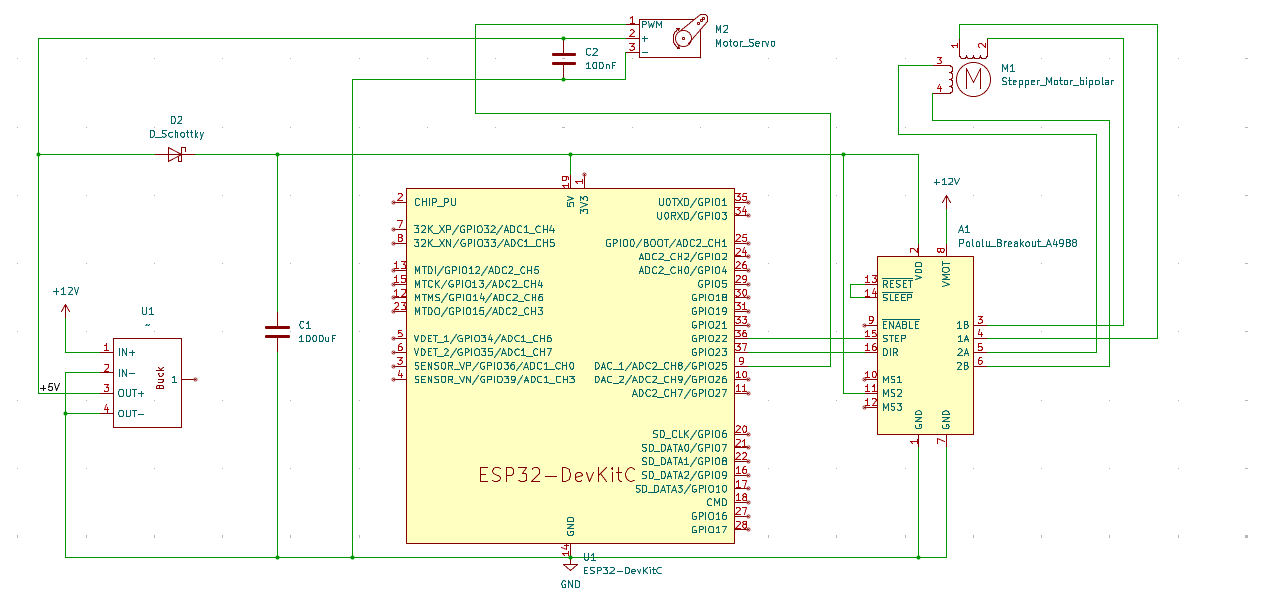
\includegraphics[width=0.85\textheight]{images/circuit_diagram.png}
    }
    \caption{Schematic Diagram of Circuit Connections}
    \label{fig:circuit_diagram}
\end{figure}
